\chapter{RESULTS AND DISCUSSION} \label{chap-result}
\thispagestyle{empty}



\section{Sensor Testing}
Voltage and current sensors placed at the input side of the DC bus were tested to calibrate their outputs and evaluate sensitivity.

\subsection{Voltage Sensor Calibration}
The voltage sensor input was connected to the DC bus and its output to the ADC pin of the STM32. Calibration was performed by comparing the actual DC bus voltage with the ADC readings.

For ease of analysis, ADC values were scaled as ADC/10. This scaling improves readability without affecting accuracy, as it is linearly reversible.

\begin{table}[H]
\centering
\caption{Real Voltage (V) vs ADC/10 Calibration Data}
\label{tab:voltageadc}
\small
\begin{tabular}{cc | cc | cc}
\toprule
\textbf{Real Voltage} & \textbf{ADC/10} & \textbf{Real Voltage} & \textbf{ADC/10} & \textbf{Real Voltage} & \textbf{ADC/10} \\ \midrule
20  & 1.5  & 180 & 128.5 & 290 & 216   \\
40  & 17.5 & 200 & 144.2 & 300 & 224.8 \\
60  & 33   & 210 & 152   & 310 & 232   \\
80  & 49.5 & 220 & 161   & 320 & 239   \\
100 & 65.5 & 230 & 168   & 330 & 248   \\
120 & 81   & 240 & 176   & 340 & 256   \\
140 & 96.5 & 250 & 184   & 350 & 264   \\
160 & 112.5& 260 & 191.9 & 354 & 267.8 \\ \bottomrule
\end{tabular}
\end{table}

The sensor exhibits a near-linear response. A small gain error is observed at higher voltages, which is corrected using a refined calibration equation suitable for the operating range (>100 V).

\begin{figure}[H]\centering
{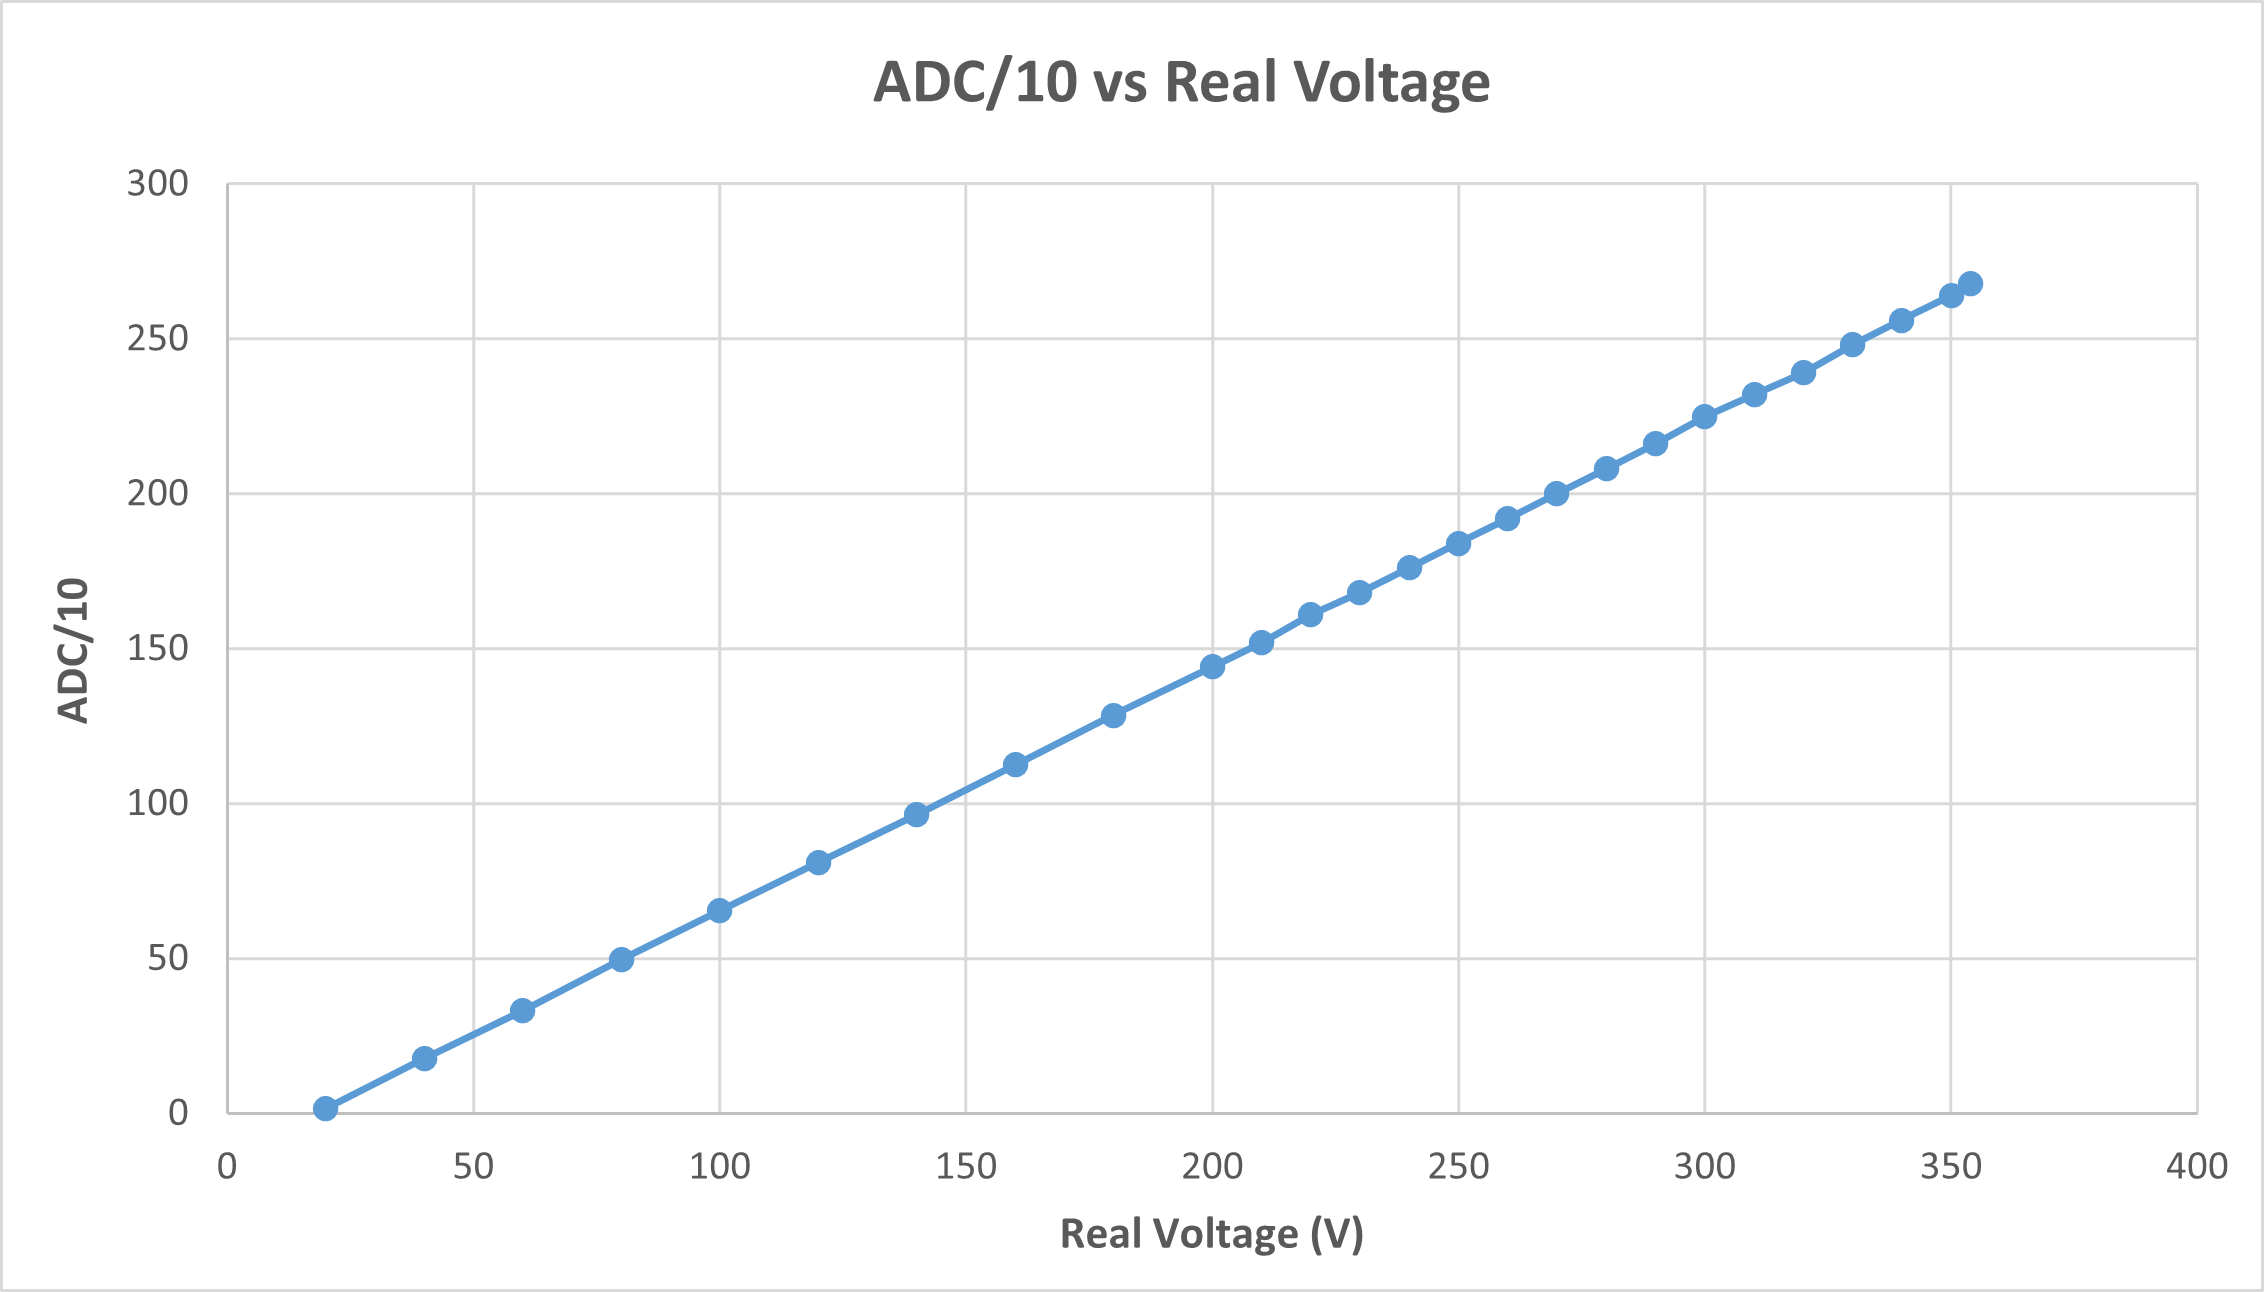
\includegraphics[width=0.85\textwidth]{./picture-files/voltagesen.png}}
 \caption{Graph of calibration of voltage sensor}
    \label{fig:voltagegraph}
\end{figure}\hfill


\subsection{Current Sensor Calibration}
The current sensor output was connected to the ADC pin of the STM32 and calibrated by comparing measured current values with ADC readings.

ADC values were again scaled as ADC/10 for simplicity and clarity in analysis.

\begin{table}[H]
\centering
\caption{Real Current (mA) vs ADC/10 Calibration data}
\label{tab:currentadc}
\small
\begin{tabular}{cc | cc | cc}
\toprule
\textbf{Current (mA)} & \textbf{ADC/10} & \textbf{Current (mA)} & \textbf{ADC/10} & \textbf{Current (mA)} & \textbf{ADC/10} \\ \midrule
100  & 1   & 1100 & 133 & 2100 & 266 \\
200  & 15  & 1200 & 147 & 2200 & 279 \\
300  & 28  & 1300 & 160 & 2300 & 292 \\
400  & 41  & 1400 & 173 & 2400 & 305 \\
500  & 54  & 1500 & 186 & 2500 & 319 \\
600  & 68  & 1600 & 200 & 2600 & 332 \\
700  & 81  & 1700 & 213 & 2700 & 345 \\
800  & 94  & 1800 & 226 & 2800 & 358 \\
900  & 107 & 1900 & 239 & 2900 & 371 \\
1000 & 120 & 2000 & 252 & 3000 & 385 \\ \bottomrule
\end{tabular}
\end{table}

The current sensor shows a strong linear relationship with a small offset at low currents, attributed to sensor and signal conditioning circuitry.

\begin{figure}[H]\centering
{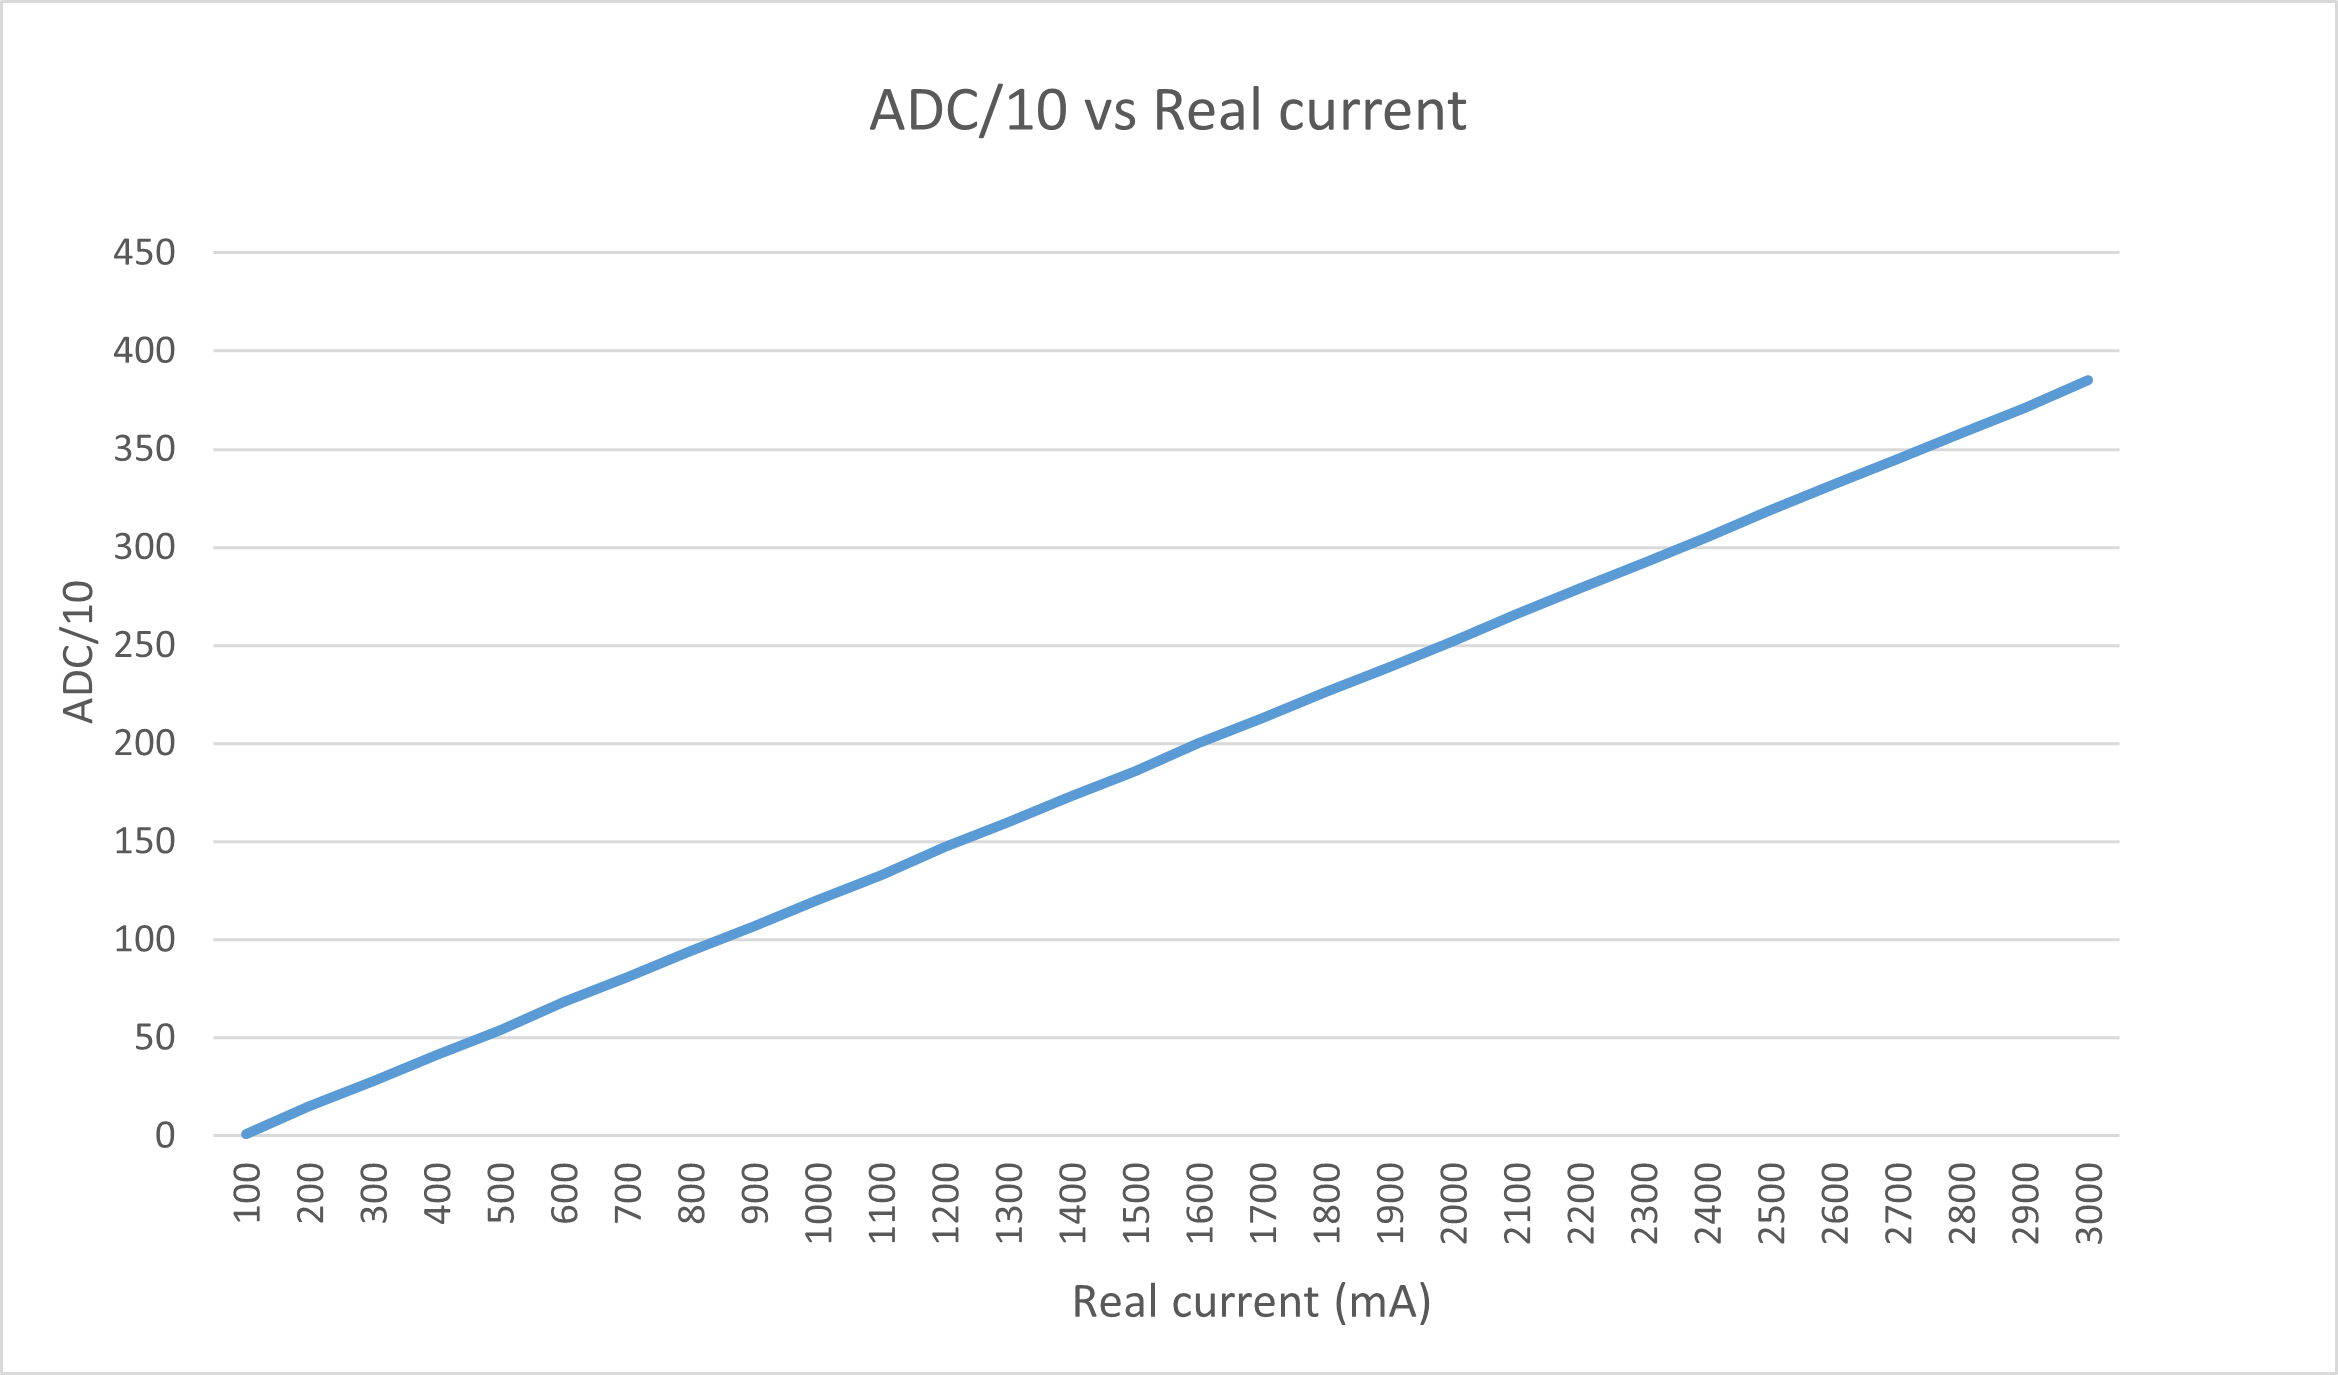
\includegraphics[width=0.85\textwidth]{./picture-files/currentgraph.png}}
 \caption{Graph of calibration of current sensor}
    \label{fig:currentgraph}
\end{figure}\hfill


\section{Inverter Testing}
The performance of the H-bridge inverter was experimentally evaluated to verify its switching behavior and output waveform, The inverter was fed with a DC voltage of 325 V and was operated at a frequency of 100 kHz. The output voltage waveform was observed using an oscilloscope.


\subsection{Initial testing phase}
The inverter was initially tested with the designed components. The inverter generated a high frequency square wave output, confirming to proper operation of MOSFET switching and the gate driver circuit. However, a significant voltage overshoot was observed at the rising edge of the output waveform. The observed values are shown in table \ref{tab:inverter_results1} and figure

\vspace{5pt}


\begin{table}[H]
\centering
\caption{Inverter output  measurement with initial design}
\label{tab:inverter_results1}
\begin{tabular}{ccccc}
\toprule
\textbf{Sl. No.} & \textbf{DC Input (V)} & \textbf{\begin{tabular}[c]{@{}c@{}}AC Out\\ (Peak-to-Peak) (V)\end{tabular}} & \textbf{AC Out (RMS) (V)} & \textbf{\begin{tabular}[c]{@{}c@{}}Percentage\\ Overshoot (\%)\end{tabular}} \\ \midrule
1 & 20.3  & 87.2 & 21.6 & 62    \\
2 & 41    & 178  & 43.6 & 65    \\
3 & 60.4  & 244  & 63   & 62.8  \\
4 & 80.3  & 292  & 82.1 & 54.37 \\
5 & 100.1 & 340  & 102  & 46.5  \\
6 & 120.2 & 376  & 122  & 40.3  \\
7 & 140   & 422  & 142  & 35    \\
8 & 160   & 456  & 162  & 27.2  \\
9 & 169   & 470  & 170  & 23.2  \\ \bottomrule
\end{tabular}
\end{table}

Due to significant overshoot, the peak voltage exceeded the measurable range of the oscilloscope, preventing accurate measurement for input voltages above 169 V.

\vspace{10pt}

The value of the output capacitor was changed from $22\mu F$ to $0.33\mu F$. The new result was observed and is shown in the table \ref{tab:inverter_results2}

\vspace{5pt}

\begin{table}[H]
\centering
\caption{Inverter output measurement (final) }
\label{tab:inverter_results2}
\begin{tabular}{ccccc}
\toprule
\textbf{Sl. No.} & \textbf{DC Input (V)} & \textbf{\begin{tabular}[c]{@{}c@{}}AC Out\\ (Peak-to-Peak) (V)\end{tabular}} & \textbf{AC Out (RMS) (V)} & \textbf{\begin{tabular}[c]{@{}c@{}}Percentage\\ Overshoot (\%)\end{tabular}} \\ \midrule
1 & 20.3 & 80  & 21   & 60   \\
2 & 40.6 & 148 & 43.1 & 51.7 \\
3 & 60.7 & 270 & 61   & 47   \\
4 & 80   & 276 & 84.2 & 41   \\
5 & 100  & 326 & 103  & 36.4 \\
6 & 120  & 390 & 123  & 33.5 \\
7 & 140  & 430 & 141  & 29.8 \\
8 & 160  & 470 & 162  & 24.5 \\
9 & 170  & 480 & 171  & 20.6 \\ \bottomrule
\end{tabular}

\end{table}

\begin{figure}[H]\centering

{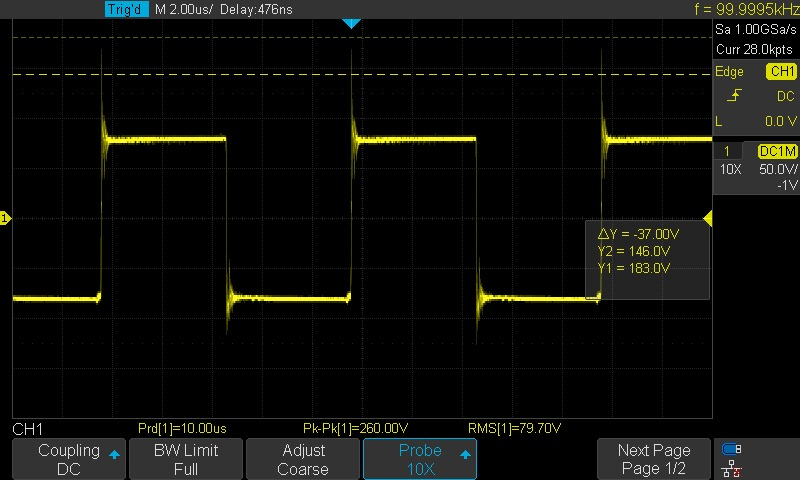
\includegraphics[width=0.85\textwidth]{./picture-files/overshoot.png}}
 \caption{Output voltage of inverter with overshoot.}
    \label{fig:inverterovershoot}
\end{figure}\hfill


Even after changing the capacitor value there wasn`t a significant reduction in the overshoot. So further design consideration were made.

\subsection{Final testing phase}

To address the overshoot issue and ensure efficient operation, the design was re-evaluated.The gate-source $R_{on}$ resistor value of the MOSFETs was increased from $10 \Omega$ to $33 \Omega$, which resulted in a significant reduction in overshoot. The output observed is shown in figure \ref{fig:inverter-final}

\begin{figure}[H]\centering

{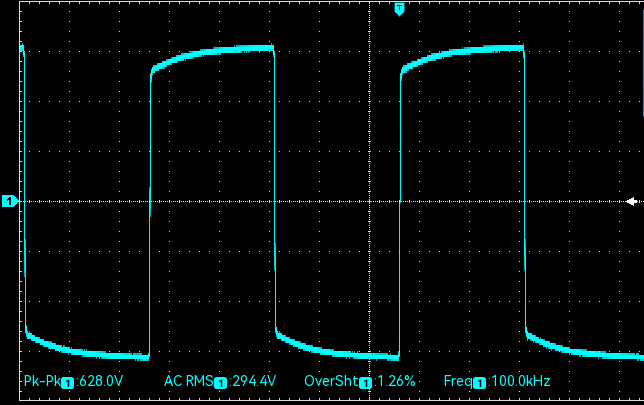
\includegraphics[width=0.85\textwidth]{./picture-files/goodvoltage.png}}
 \caption{Output voltage of inverter at 320V input, observed in oscilloscope.}
    \label{fig:inverter-final}
\end{figure}\hfill

\subsection{Inference}

The initial design showed a significant overshoot of approximately 40--60\%, indicating the presence of strong switching transients and ringing in the circuit. This was primarily due to the fast switching of the MOSFETs, which caused high $dv/dt$ and $di/dt$, along with the effects of parasitic inductances and capacitances in the circuit.

\vspace{10pt}

To mitigate this issue, the gate-on resistor ($R_{\text{on}}$) of the MOSFETs was increased from $10\,\Omega$ to $33\,\Omega$. Increasing this resistance effectively slowed down the charging and discharging of the MOSFET gate capacitance, resulting in a controlled switching speed. This reduction in switching speed lowered the rate of voltage and current change, thereby reducing the severity of transient spikes and damping the oscillations caused by parasitic elements.

\vspace{10pt}

As a result, a noticeable reduction in overshoot was achieved, leading to smoother waveform characteristics, improved stability, and enhanced reliability of the overall system. This modification demonstrates the importance of proper gate drive design in controlling switching behavior and minimizing unwanted transients in power electronic circuits.

\section{Transformer testing}
The transformer was tested to evaluate its performance under open-loop conditions. The input supply was provided from the transformer output, and the system behavior was observed without any feedback control. This setup allowed for the analysis of voltage characteristics, waveform quality, and transient responses of the transformer under varying operating conditions. 

\subsection{Primary waveform}
The primary waveform of the transformer was observed with an oscilloscope.
The observed waveform is shown in figure \ref{fig:transpri}
\begin{figure}[H]\centering

{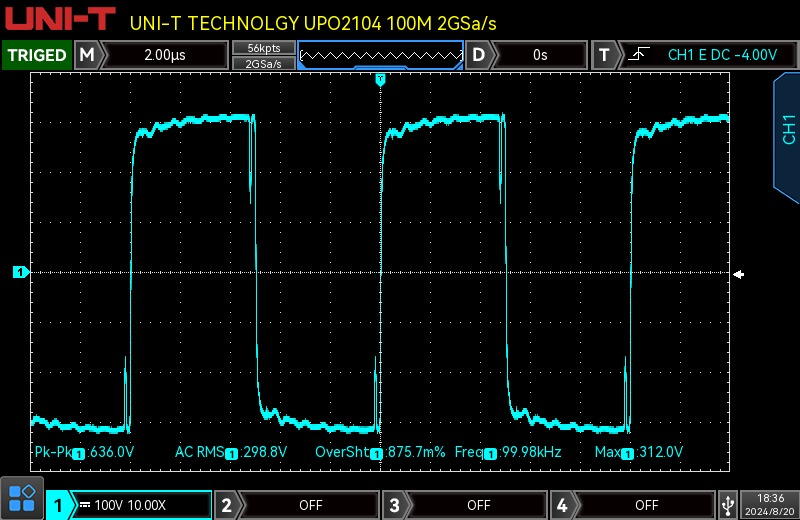
\includegraphics[width=0.85\textwidth]{./picture-files/primarytrans.jpeg}}
 \caption{Primary voltage of transformer, observed in oscilloscope.}
    \label{fig:transpri}
\end{figure}\hfill

\subsection{Temperature of the core and copper winding}
During the testing of transformer we have also observed the temperature of the core and winding. The temperature was measured at an interval of 1 minute at 320V input for a period of 15 minutes. The observed values are shown in table \ref{tab:temp_variation} and a graph is plotted \ref{fig:temptime}

\begin{table}[h!]
\centering
\caption{Core and Copper Temperature Variation over Time}
\label{tab:temp_variation}
\begin{tabular}{ccc}
\toprule
\textbf{Time (min)} & \textbf{Core Temperature ($^\circ$C)} & \textbf{Copper Temperature ($^\circ$C)} \\ \midrule
1  & 39.3 & 37.2 \\
2  & 42.1 & 39.0 \\
3  & 44.7 & 41.0 \\
4  & 47.2 & 42.5 \\
5  & 48.7 & 41.2 \\
6  & 50.0 & 41.3 \\
7  & 52.5 & 41.8 \\
8  & 53.5 & 42.8 \\
9  & 57.1 & 45.6 \\
10 & 57.6 & 46.3 \\
11 & 58.6 & 49.0 \\
12 & 61.1 & 49.5 \\
13 & 62.0 & 50.3 \\
14 & 62.5 & 52.0 \\
15 & 62.9 & 53.0 \\ \bottomrule
\end{tabular}
\end{table}
\begin{figure}[H]\centering
{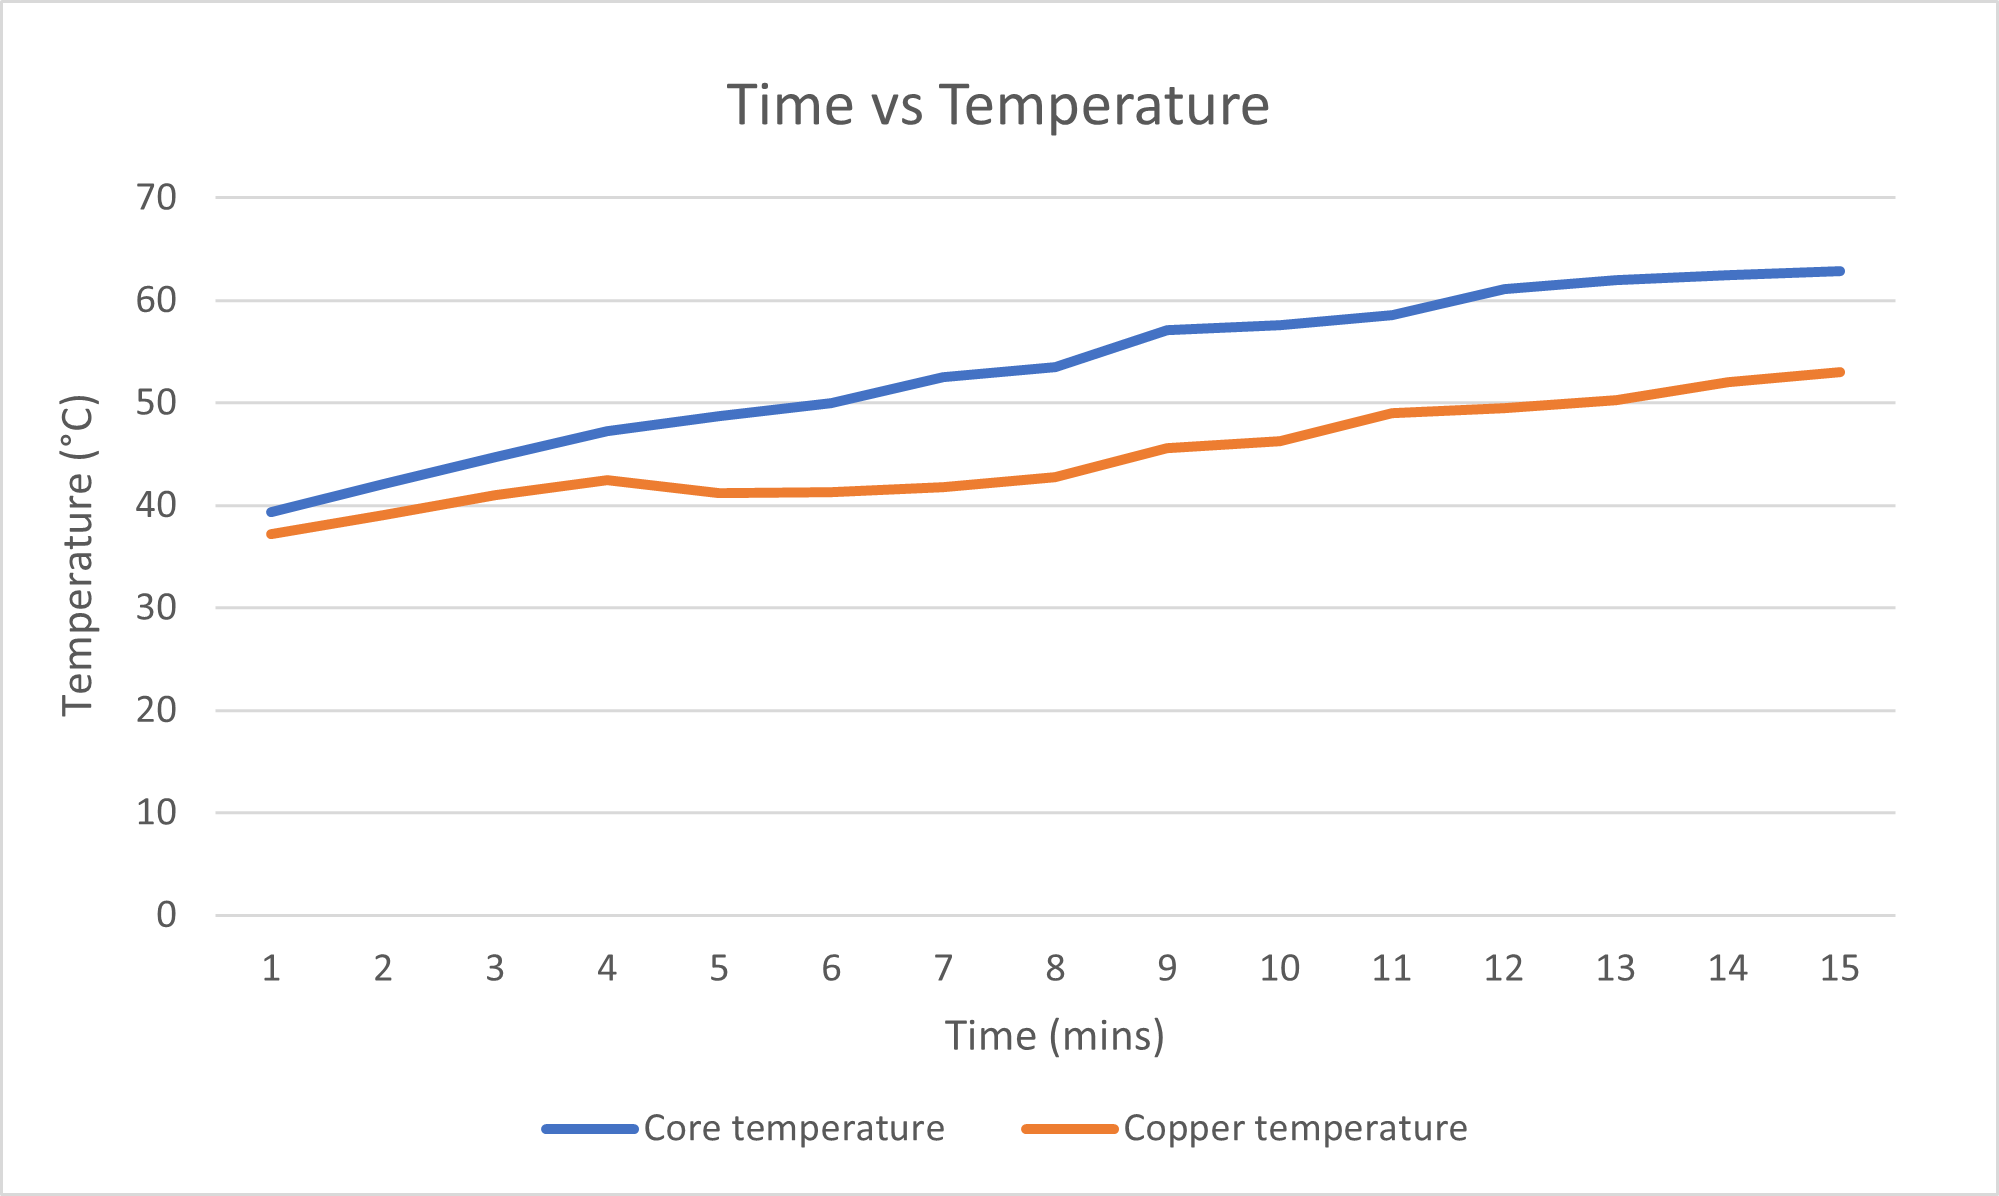
\includegraphics[width=0.85\textwidth]{./picture-files/temptime.png}}
 \caption{Temperature vs Time graph}
    \label{fig:temptime}
\end{figure}\hfill





\newpage

\section{Additional Discussions}

The circuit we designed performed well at voltages below 48~V. Using low-power transformers and the voltage multiplier, we were able to generate 30~kV DC. However, we encountered issues with ringing, which could be reduced by adding a polypropylene capacitor to the HVDC link. We plan to further minimize these oscillations to eliminate high-voltage peaks that could damage the components. The next phase of the project involves designing an improved power transformer and developing the mechanical assembly, along with sourcing argon gas to produce cold plasma, the ultimate objective of this project.



\section{Summary}

In this semester, we began with a literature survey on the topic and finalized the specifications for the desired output. We then designed a half-bridge MOSFET driver using the UCC21330 IC and subsequently developed an H-bridge system based on this driver. The LaunchXL-F28379D board was used to generate the PWM signals required to drive the MOSFETs, producing a square-wave output that powered a low-power transformer. Additionally, we designed a voltage multiplier capable of generating 30~kV DC. The PCBs for both the UCC driver and the H-bridge were designed and sent to the manufacturer for fabrication.

